\documentclass[border=10pt]{standalone}
\usepackage{tikz}
\usetikzlibrary{automata, positioning, arrows.meta}

\begin{document}
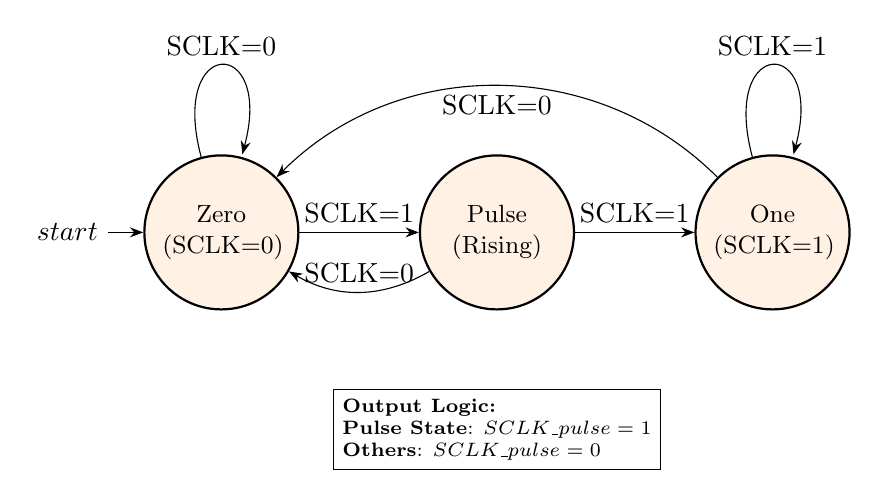
\begin{tikzpicture}[
    ->, >=Stealth, auto, node distance=3.5cm,
    every state/.style={thick, fill=orange!10, text width=1.5cm, align=center, font=\small},
    initial text=$start$
]

    % States
    \node[state, initial] (zero) {Zero\\(SCLK=0)};
    \node[state, right of=zero] (pulse) {Pulse\\(Rising)};
    \node[state, right of=pulse] (one) {One\\(SCLK=1)};

    % Transitions
    
    % Zero State
    \path (zero) edge[loop above] node {SCLK=0} (zero)
                 edge node {SCLK=1} (pulse);
                 
    % Pulse State
    % Output = 1 here (Moore) or transition output (Mealy)
    % Let's assume Moore output for state "Pulse" is 1.
    % In Pulse state, SCLK is 1. 
    % We go to One immediately on next cycle if SCLK is still 1.
    % If SCLK drops to 0 immediately (glitch?), go back to Zero.
    \path (pulse) edge node {SCLK=1} (one)
                  edge[bend left] node[above] {SCLK=0} (zero);
                  
    % One State
    \path (one) edge[loop above] node {SCLK=1} (one)
                edge[bend right=45] node {SCLK=0} (zero);

    % Legend / output
    \node[draw, rectangle, fill=white, align=left, font=\scriptsize, below=1cm of pulse] (legend) {
        \textbf{Output Logic:}\\
        \textbf{Pulse State}: $SCLK\_pulse = 1$\\
        \textbf{Others}: $SCLK\_pulse = 0$
    };

\end{tikzpicture}
\end{document}
